
\documentclass[a4paper]{article}
\usepackage[spanish]{babel}

\usepackage[backend=biber,
style=apa,
]{biblatex}

\defbibenvironment{bibliography}
  {\enumerate
     {}
     {\setlength{\leftmargin}{\bibhang}%
      \setlength{\itemindent}{-\leftmargin}%
      \setlength{\itemsep}{\bibitemsep}%
      \setlength{\parsep}{\bibparsep}}}
  {\endenumerate}
  {\item}


\usepackage{caption} % Para poner captions the multiples renglones
\usepackage{float} % Para colocar las imágenes
\usepackage{fullpage} % Package to use full page


\usepackage{parskip} % Package to tweak paragraph skipping
\usepackage{tikz} % Package for drawing
\usepackage{amsmath}
\usepackage{csquotes}

\usepackage{graphicx} % Para instertar pdfs como imágenes y usar \scalebox

\newcommand*{\Scale}[2][4]{\scalebox{#1}{$#2$}}%
\newcommand*{\Resize}[2]{\resizebox{#1}{!}{$#2$}}%

\usepackage{minted} % Para colocar código
\usemintedstyle{bw} % Para usar blanco y negro como colores de código

\renewcommand{\figurename}{Figura}
\renewcommand{\tablename}{Tabla}
\renewcommand\listingscaption{Listado}


\addbibresource{bibliography.bib}
\begin{document}

\hspace{0pt}
\vfill

\begin{center}
    {\huge Aplicación del Álgebra Lineal:\\Ofuscación binaria}\\    \quad\\
    {\large Universidad Panamericana}\\
    {\large Facultad de Ingeniería}\\
    \quad\\
    \quad\\
    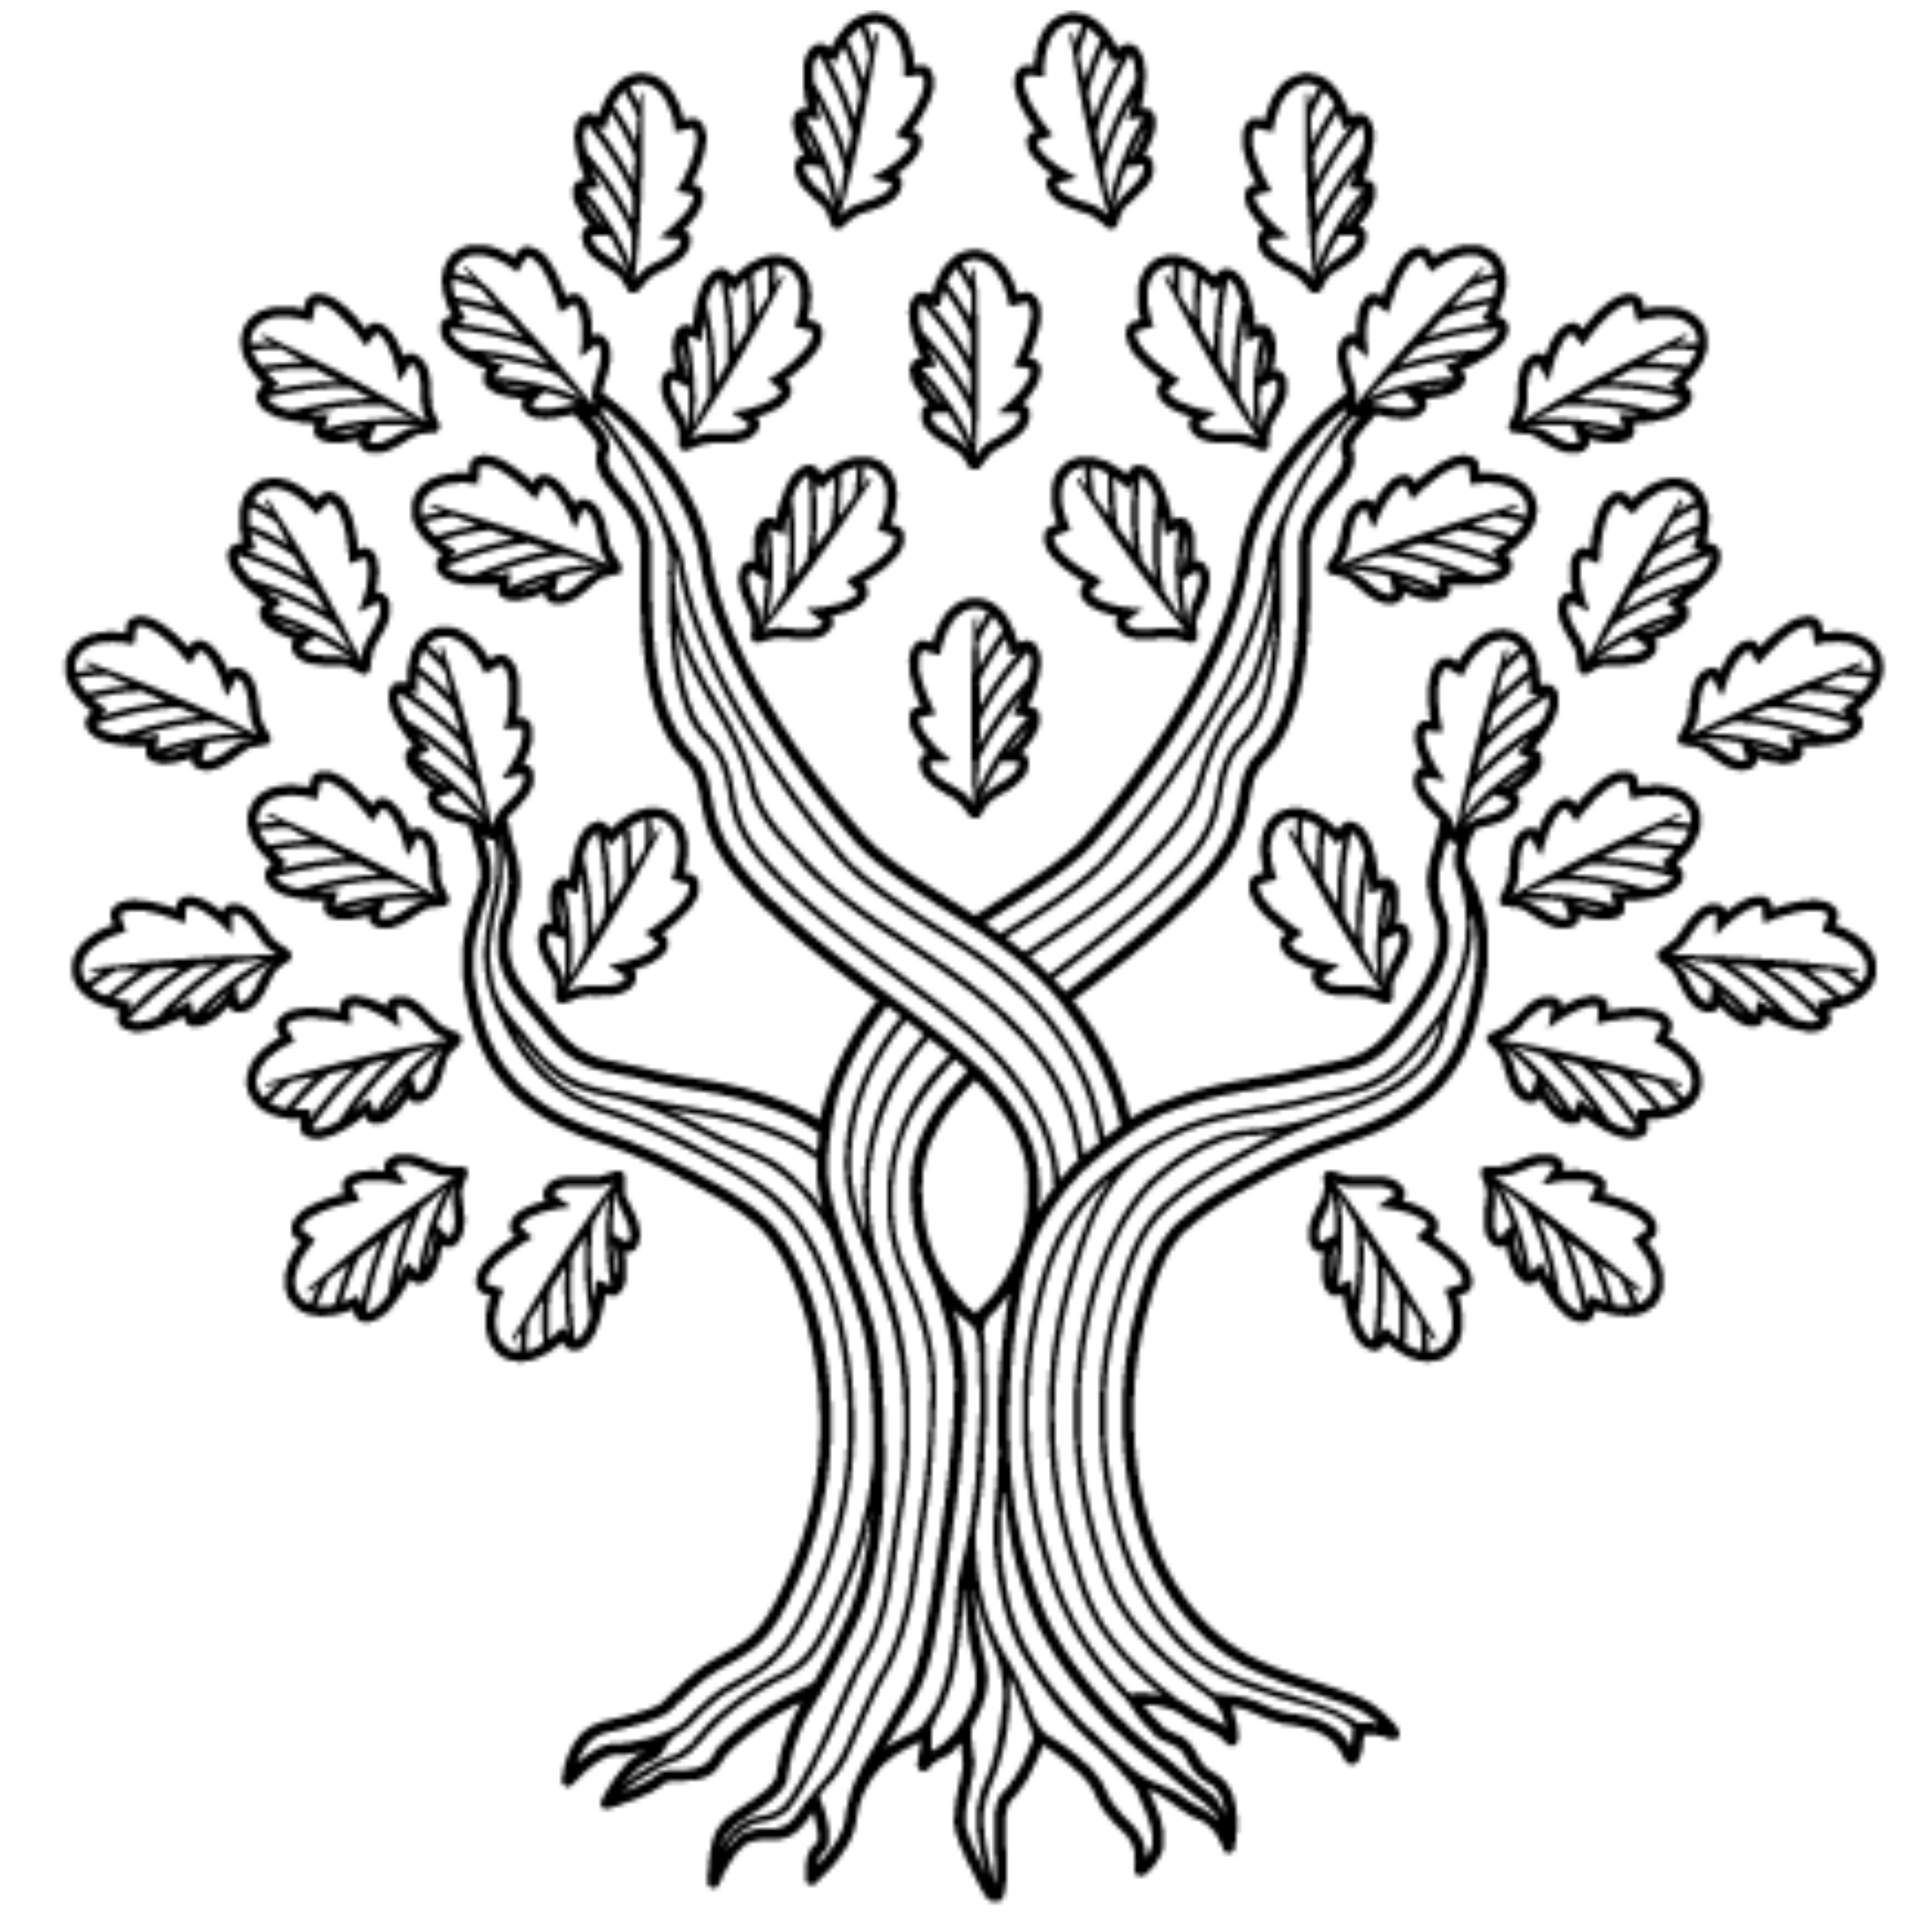
\includegraphics[scale=0.3]{UP}
    \quad\\
    \quad\\
    Álgebra Lineal\\
    Prof. Miguel Angel Quintero Zamarron\\
    \quad\\
    \quad\\
    \begin{tabular}{c|c}
        Osornio López Daniel Alejandro & 0244685\\
        Paredes García Ricardo & 0241528\\
        Rodrigo Peña Díaz Barriga & idididid\\
    \end{tabular}\\
    \quad\\
    \quad\\
\end{center}

\vfill
\newpage

\section{Objetivos}

1. Diseño de un algoritmo de cifrado que utilice como herramienta principal el
álgebra lineal

2. Creación de un ejecutable de ofuscación de archivos

\quad 2.1. Implementación de una librería de cifrado de archivos en Rust

\quad 2.2. Empleo de libreria para la ofuscación de archivos binarios y de
texto

\quad 2.3. Verificación de ofuscación con herramientas de ingeniería inversa

\section{Resumen}

El objetivo de este proyecto es utilizar transformaciones lineales como llaves
para cifrar y descifrar bits de información.
Se explora el uso de la aritmética modular para mantener la congruencia de la
información
 a la vez que se experimenta con distintos métodos de cifrado por medio de
algoritmos varios que emplean las transformaciones en su proceso.
La meta es implementar una herramienta de cifrado y descifrado que pueda
proteger tanto archivos de texto como ejecutables con un procedimiento
que permita su auto descifrado junto con soporte a \textit{passphrases} para
obtener mayor seguridad.

Los métodos estudiados son dos. 

El primero es una modificación de un cifrado de sustitución. Primero se
construye una matriz que contiene todos los valores representables en un 
byte y modifica la matriz por medio de multiplicaciones matriciales para
después sustituir cada byte en el archivo por su nuevo valor. 

El segundo, ordena todos los bytes del mensaje a cifrar, como puede ser un
archivo, y le aplica una multiplicación matricial a la totalidad del archivo. 

Para dar soporte al auto-descifrado de los archivos, cuando se utilice la
bandera --auto, se almacenan en el archivo los valores para descifrarse a sí
mismo, 
con bytes de meta información que facilitan el proceso y permiten una mayor
seguridad lograda por el factor aleatorio. Este proyecto plantea la
implementación 
de una librería de cifrado de archivos por medio de una ofuscación binaria
lograda por transformaciones.

\newpage

\section{Introducción}

Como estudiantes de la carrera de Inteligencia de Datos y Ciberseguridad,
decidimos desarrollar el proyecto sobre un tema que permite darnos una noción
del funcionamiento de las computadoras al desarrollar un sistema que se
encargue de cifrar archivos de todo tipo, modificando los bytes del mismo por
los que una transformación lineal dicte.

Antes de empezar a programar nada, desarrollaremos el algoritmo de cifrado que
emplearemos haciendo uso de Mathematica 13; describiremos los conceptos
necesarios para llegar a dicho procedimiento y los patrones que contiene para
analizar si es posible su cifrado de forma sencilla.

Una vez tengamos listo el algoritmo, implementaremos una librería de uso
general para el cifrado de arreglos de bytes utilizando el lenguaje de programación
Rust. Decidimos emplearlo debido a la facilidad que tiene en su
sintaxis sumada con las operaciones de bajo nivel que permite realizar con la
computadora sin necesidad de producir código complejo como pasaría con
C/C++.

Verificaremos que la librería es estable y arroja como resultado el archivo
exacto que se tenía antes de ser cifrado. Una ventaja de analizarlos
como arreglos de bytes, es que da igual el \textit{encoding} con el que cuente
el mismo, por lo que la librería es amigable con ejecutables, imágenes, etc.

La librería contará con el soporte para cifrar ejecutables, ofreciendo una
manera de que se autodescifren sin exponer de manera explícita la manera en que
lo hacen.

Por último, usaremos la librería para programar una aplicación de la línea
de comandos que cifra archivos de todo tipo.

Este es un tema altamente experimental, por lo que se espera encontrar
limitaciones en el camino.

\newpage

\section{Marco Teórico}

Todo en las computadoras es representado por los valores 0 y 1 debido a que
funcionan con el estado o no de un componente, con la presencia o no de
energía.
A una unidad que puede valer verdadero (1) o falso (0) s le conoce como bit.
Los bits son la unidad más pequeña de información en las ciencias de la
computación.

A un grupo de 8 bits se les agrupa. A esta agrupación se le conoce como byte.

Un byte puede contener $2^8$ combinaciones distintas de bits. Por ejemplo:

\[
\begin{array}{ccc}
    01000111 & 011111111 & 0000000
\end{array}
\]

Los bits en un byte pueden representar cualquier cantidad entre el 0 al 255 si
se interpretan como números binarios no firmados. Efectivamente, formando 256
combinaciones diferentes.

Las computadoras entienden la información de distinta forma a los humanos.
Estas interpretan bytes que resultan en instrucciones para la CPU; en
caracteres de
un archivo de texto, en piezas para armar una imagen, en direcciones de memoria
y en cualquier dato que se procese, almacene o ejecute en las mismas.

La forma en que una computadora interpreta se define con las instrucciones que
tiene su CPU, su unidad central de procesamiento.
Cada una cuenta con instrucciones distintas, como son los procesadores Intel o
Ryzen.

La manera en que se moldearon las compuertas lógicas dentro de un procesador
hará que el valor, por poner un ejemplo, 47 sea el que
indique a la máquina que realizara una suma y que por ende debe tomar los
siguientes dos valores para sumarlos.

Así como la computadora necesita entender los bytes con las instrucciones que
tiene definidas, los humanos que entiendan las instrucciones
y la CPU, pueden entender el funcionamiento de todo lo que sucede dentro de
ella.

Por ello es necesario proteger la información, desde archivos de texto como


\[
\Scale[0.5]{
\left(
\begin{array}{ccccccccc}
 0 & 1 & 2 & \dots & 29 & 30 & 31 \\
 32 & 33 & 34 & \dots & 61 & 62 & 63
\\
 64 & 65 & 66 & \dots & 93 & 94 & 95
\\
 96 & 97 & 98 & \dots & 125 & 126 & 127 \\
 128 & 129 & 130 & \dots & 157 & 158 & 159 \\
 160 & 161 & 162 & \dots & 189 & 190 & 191 \\
 192 & 193 & 194 & \dots & 221 & 222 & 223 \\
 224 & 225 & 226 & \dots & 253 & 254 & 255 \\
\end{array}
\right)
}
\]

\[
\Scale[0.5]{
\left(
\begin{array}{cccccccccccccccccccccccccccccccc}
 0 & 1 & 2 & 3 & 4 & 5 & 6 & 7 & 8 & 9 & 10 & 11 & 12 & 13 & 14 & 15 & 16 & 17
& 18 & 19 & 20 & 21 & 22 & 23 & 24 & 25 & 26 & 27 & 28 & 29 & 30 & 31 \\
 32 & 33 & 34 & 35 & 36 & 37 & 38 & 39 & 40 & 41 & 42 & 43 & 44 & 45 & 46 & 47
& 48 & 49 & 50 & 51 & 52 & 53 & 54 & 55 & 56 & 57 & 58 & 59 & 60 & 61 & 62 & 63
\\
 64 & 65 & 66 & 67 & 68 & 69 & 70 & 71 & 72 & 73 & 74 & 75 & 76 & 77 & 78 & 79
& 80 & 81 & 82 & 83 & 84 & 85 & 86 & 87 & 88 & 89 & 90 & 91 & 92 & 93 & 94 & 95
\\
 96 & 97 & 98 & 99 & 100 & 101 & 102 & 103 & 104 & 105 & 106 & 107 & 108 & 109
& 110 & 111 & 112 & 113 & 114 & 115 & 116 & 117 & 118 & 119 & 120 & 121 & 122 &
123 & 124 & 125 & 126 & 127 \\
 128 & 129 & 130 & 131 & 132 & 133 & 134 & 135 & 136 & 137 & 138 & 139 & 140 &
141 & 142 & 143 & 144 & 145 & 146 & 147 & 148 & 149 & 150 & 151 & 152 & 153 &
154 & 155 & 156 & 157 & 158 & 159 \\
 160 & 161 & 162 & 163 & 164 & 165 & 166 & 167 & 168 & 169 & 170 & 171 & 172 &
173 & 174 & 175 & 176 & 177 & 178 & 179 & 180 & 181 & 182 & 183 & 184 & 185 &
186 & 187 & 188 & 189 & 190 & 191 \\
 192 & 193 & 194 & 195 & 196 & 197 & 198 & 199 & 200 & 201 & 202 & 203 & 204 &
205 & 206 & 207 & 208 & 209 & 210 & 211 & 212 & 213 & 214 & 215 & 216 & 217 &
218 & 219 & 220 & 221 & 222 & 223 \\
 224 & 225 & 226 & 227 & 228 & 229 & 230 & 231 & 232 & 233 & 234 & 235 & 236 &
237 & 238 & 239 & 240 & 241 & 242 & 243 & 244 & 245 & 246 & 247 & 248 & 249 &
250 & 251 & 252 & 253 & 254 & 255 \\
\end{array}
\right)
}
\]

\section{Experimentación}

\subsection{Método 1}

Para el primer algoritmo de cifrado tenemos una matriz que contiene todos los
valores del 0 al 255, que representan todos los valores posibles representables
en un byte.

\[
\text{Bytes} := \Scale[0.5]{
\left(
\begin{array}{cccccccccccccccccccccccccccccccc}
 0 & 1 & 2 & 3 & 4 & 5 & 6 & 7 & 8 & 9 & 10 & 11 & 12 & 13 & 14 & 15 & 16 & 17
& 18 & 19 & 20 & 21 & 22 & 23 & 24 & 25 & 26 & 27 & 28 & 29 & 30 & 31 \\
 32 & 33 & 34 & 35 & 36 & 37 & 38 & 39 & 40 & 41 & 42 & 43 & 44 & 45 & 46 & 47
& 48 & 49 & 50 & 51 & 52 & 53 & 54 & 55 & 56 & 57 & 58 & 59 & 60 & 61 & 62 & 63
\\
 64 & 65 & 66 & 67 & 68 & 69 & 70 & 71 & 72 & 73 & 74 & 75 & 76 & 77 & 78 & 79
& 80 & 81 & 82 & 83 & 84 & 85 & 86 & 87 & 88 & 89 & 90 & 91 & 92 & 93 & 94 & 95
\\
 96 & 97 & 98 & 99 & 100 & 101 & 102 & 103 & 104 & 105 & 106 & 107 & 108 & 109
& 110 & 111 & 112 & 113 & 114 & 115 & 116 & 117 & 118 & 119 & 120 & 121 & 122 &
123 & 124 & 125 & 126 & 127 \\
 128 & 129 & 130 & 131 & 132 & 133 & 134 & 135 & 136 & 137 & 138 & 139 & 140 &
141 & 142 & 143 & 144 & 145 & 146 & 147 & 148 & 149 & 150 & 151 & 152 & 153 &
154 & 155 & 156 & 157 & 158 & 159 \\
 160 & 161 & 162 & 163 & 164 & 165 & 166 & 167 & 168 & 169 & 170 & 171 & 172 &
173 & 174 & 175 & 176 & 177 & 178 & 179 & 180 & 181 & 182 & 183 & 184 & 185 &
186 & 187 & 188 & 189 & 190 & 191 \\
 192 & 193 & 194 & 195 & 196 & 197 & 198 & 199 & 200 & 201 & 202 & 203 & 204 &
205 & 206 & 207 & 208 & 209 & 210 & 211 & 212 & 213 & 214 & 215 & 216 & 217 &
218 & 219 & 220 & 221 & 222 & 223 \\
 224 & 225 & 226 & 227 & 228 & 229 & 230 & 231 & 232 & 233 & 234 & 235 & 236 &
237 & 238 & 239 & 240 & 241 & 242 & 243 & 244 & 245 & 246 & 247 & 248 & 249 &
250 & 251 & 252 & 253 & 254 & 255 \\
\end{array}
\right)
}
\]

P Ara este método, cambiaremos el orden de los valores aplicándole
transformaciones a \texttt{Bytes}

Sea $A^T$ una transformación que se le aplica a \texttt{Bytes}, $A^T$ debe
seguir
las siguientes reglas:

\begin{enumerate}
    \item La transformación que afecte a $C_x$ también debe afectar a $C_y$,
donde $y$ es igual a $m-(x-1)$\label{eq:cond1}, donde $m$ es el número de
columnas (31) de \texttt{Bytes}
\end{enumerate}

Si \eqref{eq:cond1} no se cumple, obtenemos pérdidas de información que hacen
imposible el descifrado del \textit{ciphertext}

\begin{figure}[H]
    \centering
    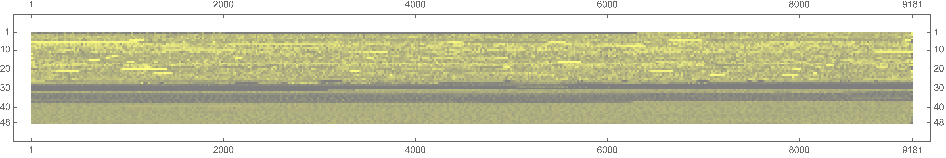
\includegraphics[width=\textwidth]{gr3d}
    \caption{Visualización de los bytes del archivo
original. $M$}
    \label{fig:DatosOrigM1}
\end{figure}

\begin{figure}[H]
    \centering
    
\includegraphics[width=\textwidth]{bytes2}
    \caption{Visualización de los bytes del archivo
cifrado. $N$}
    \label{fig:DatosOrigM2}
\end{figure}

\begin{figure}[H]
    \centering
    
\includegraphics[width=\textwidth]{bytes3}
    \caption{$M-N$}
    \label{fig:DatosOrigM3}
\end{figure}

La mayor vulnerabilidad que presenta este método de cifrado es que la
frecuencia de bytes presentes es la misma debido a que no estamos
sacrificando ninguna pérdida de información y, por lo tanto, solo sustituimos los
valores.

\begin{figure}[H]
    \centering
    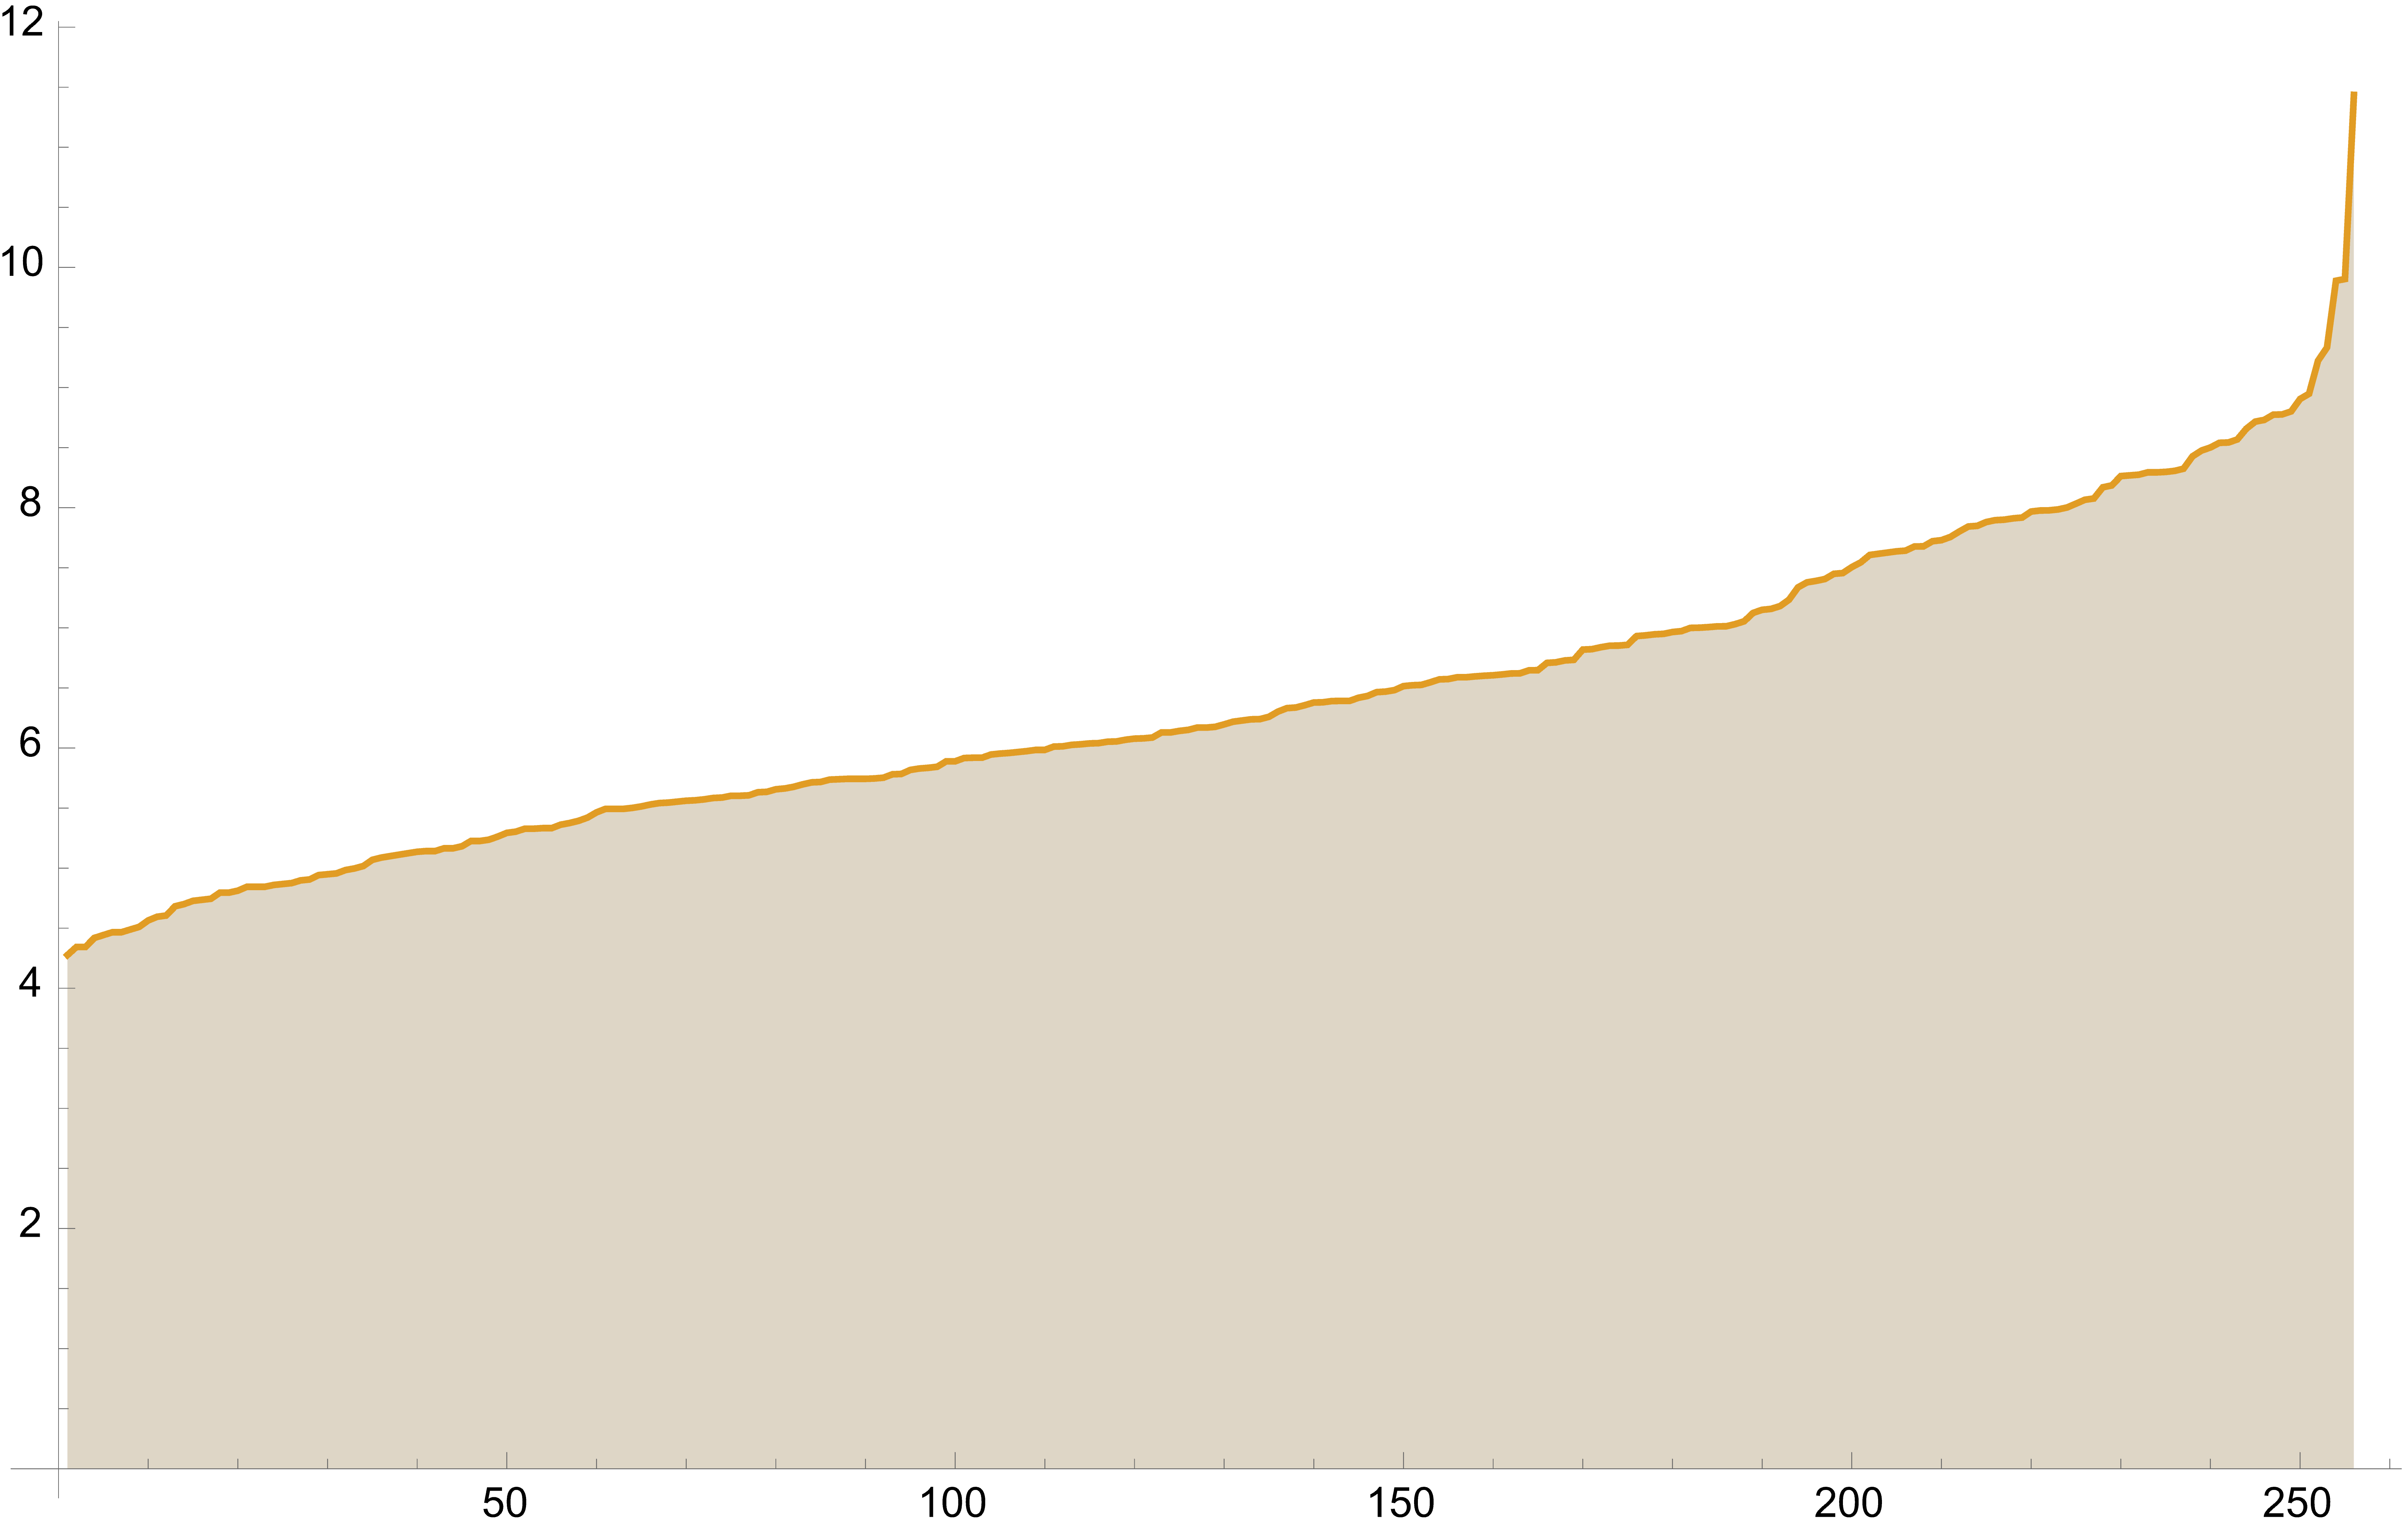
\includegraphics[width=\textwidth]{historygram.png}
    \caption{Histograma de los bytes del archivo
original y el cifrado.}
    \label{fig:Histo1}
\end{figure}

E N la figura \ref{fig:Histo1}, se muestra la sobre posición de los histogramas
de bytes del documento antes y después de cifrado. Ambos son idénticos. Si el
documento está escrito en Inglés o contuviera las instrucciones de cierta
arquitectura, y se conoce la frecuencia de bytes, el mensaje puede ser
descifrado.


\printbibliography

\newpage

\appendix

\section*{Appendix A}

Comparación de histograma de las ocurrencias de bytes entre un arreglo de bytes
y su versión cifrada por el \texttt{Método 1}

\begin{figure}[H]
    \centering
    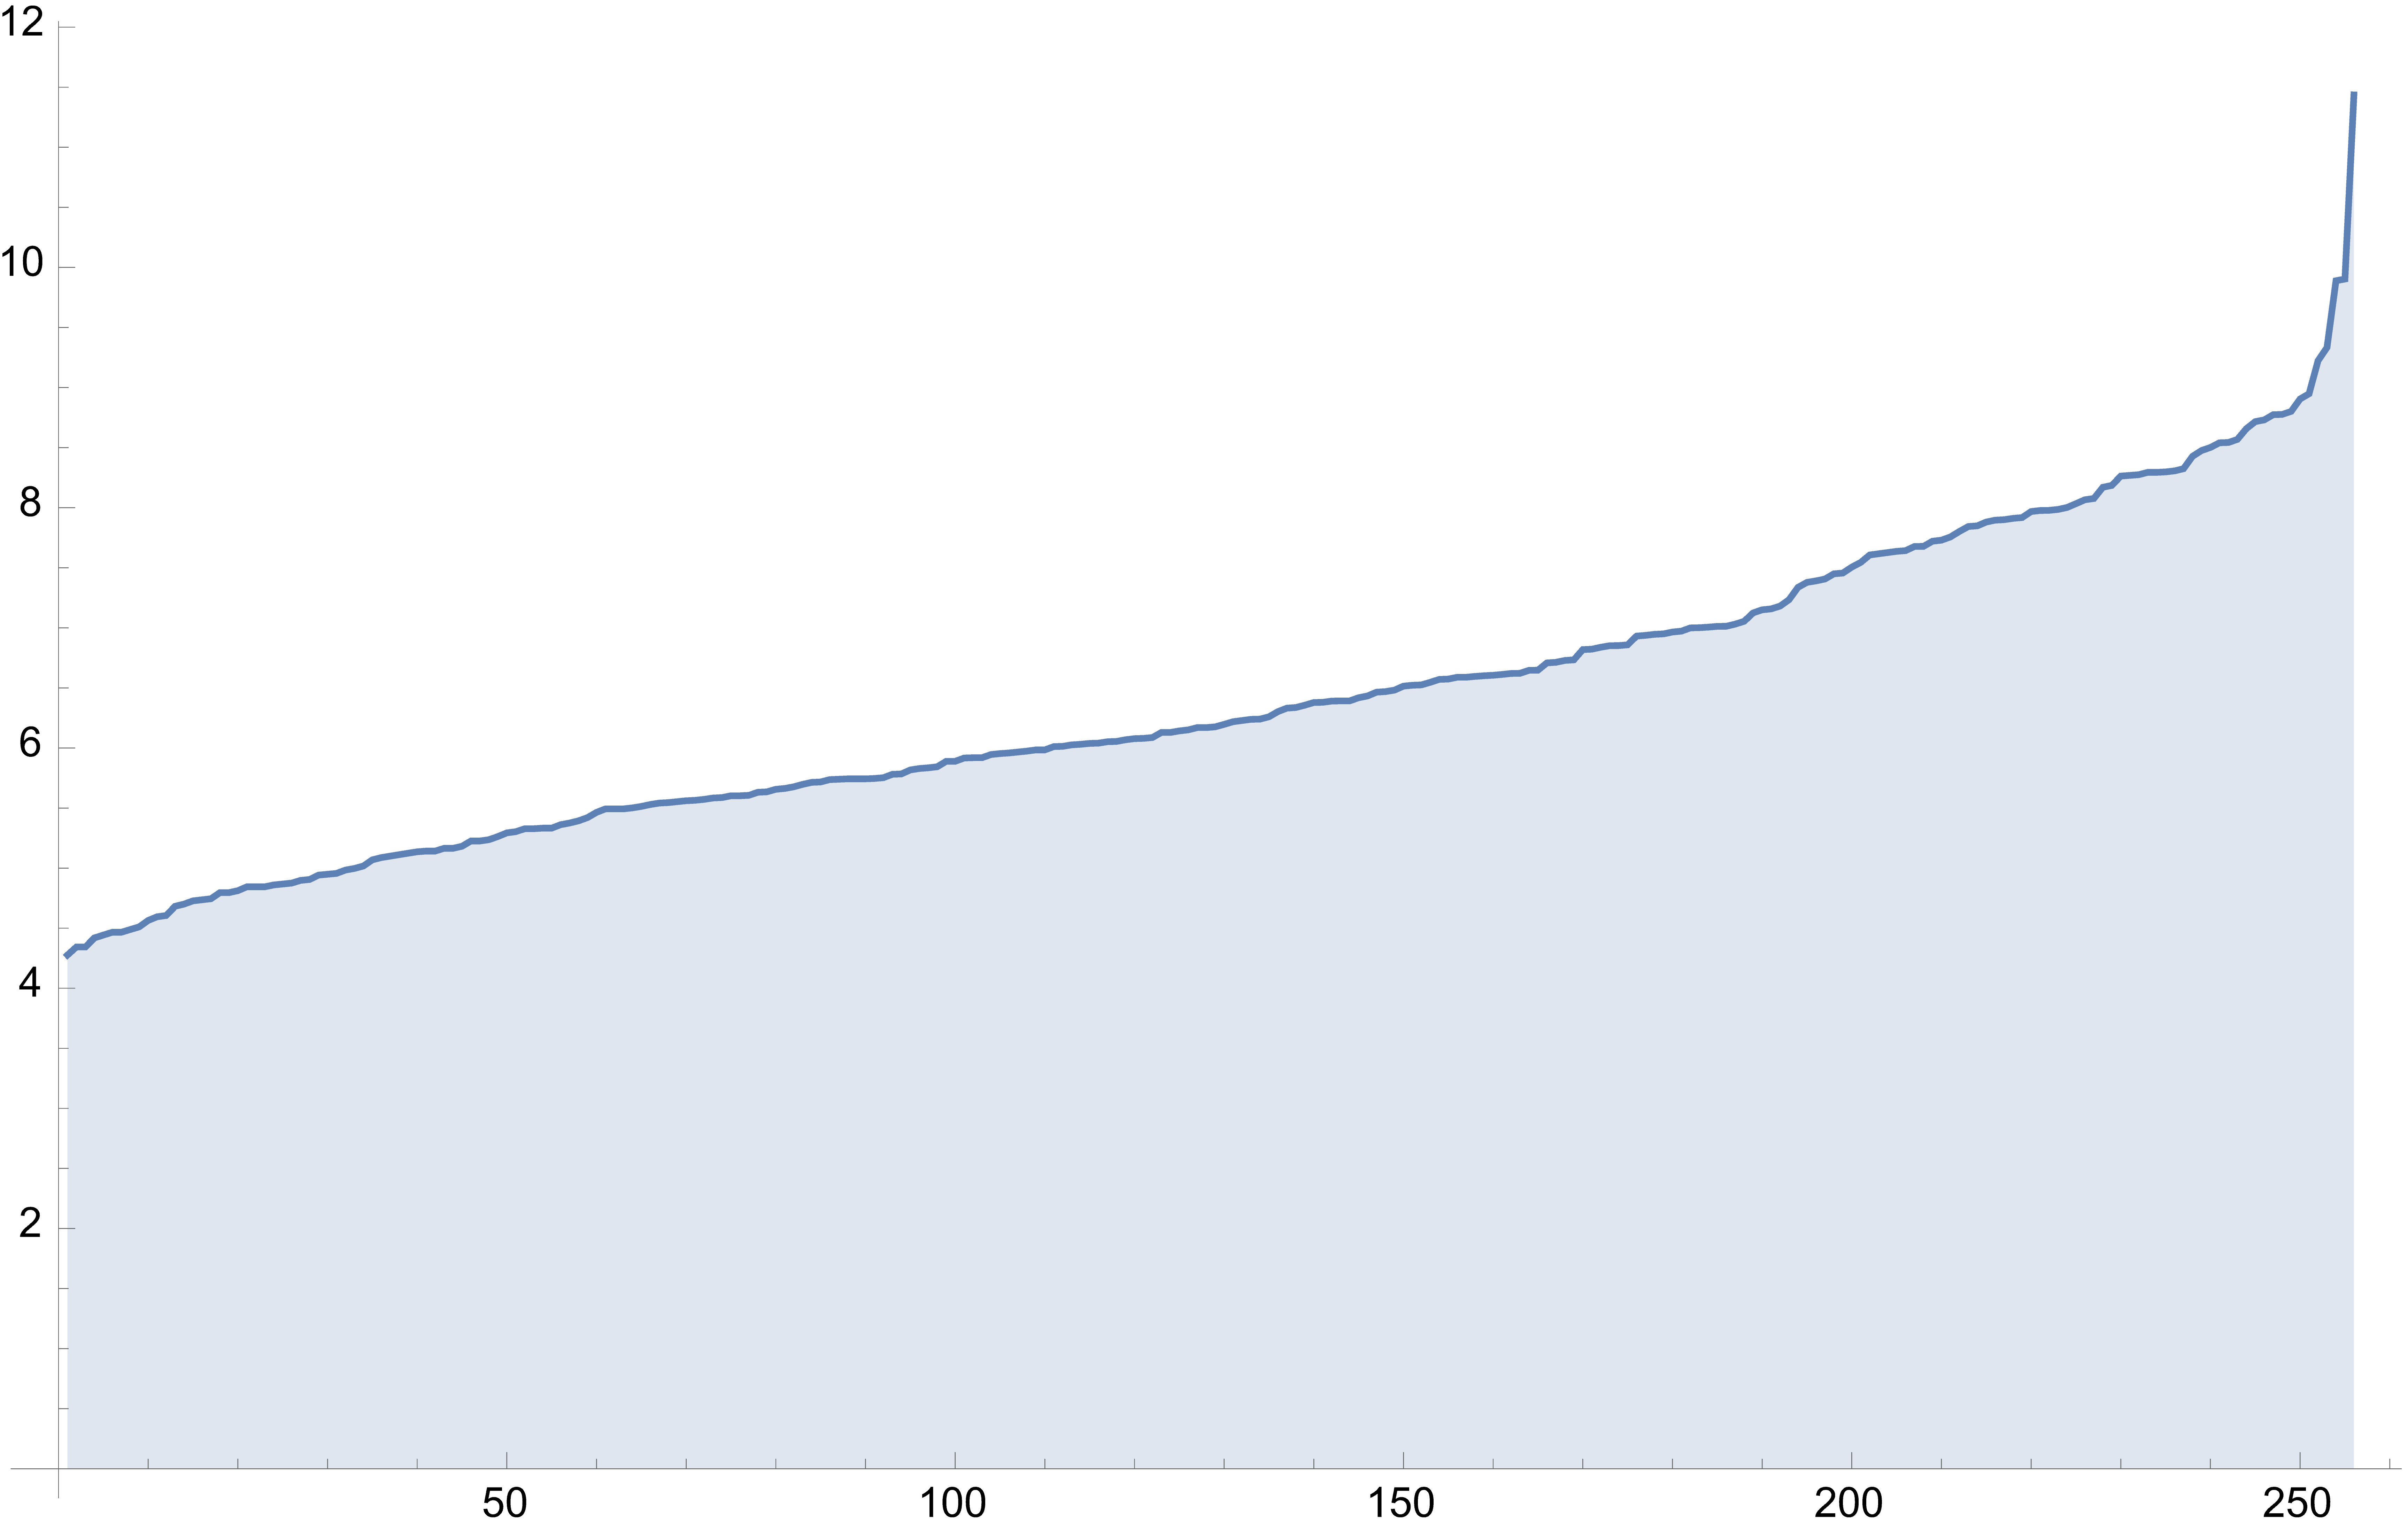
\includegraphics[scale=0.7]{historygramorig}
    \caption*{Histograma de los bytes del archivo
original y el cifrado.}\label{fig:d1}
\end{figure}

\begin{figure}[H]
    \centering
    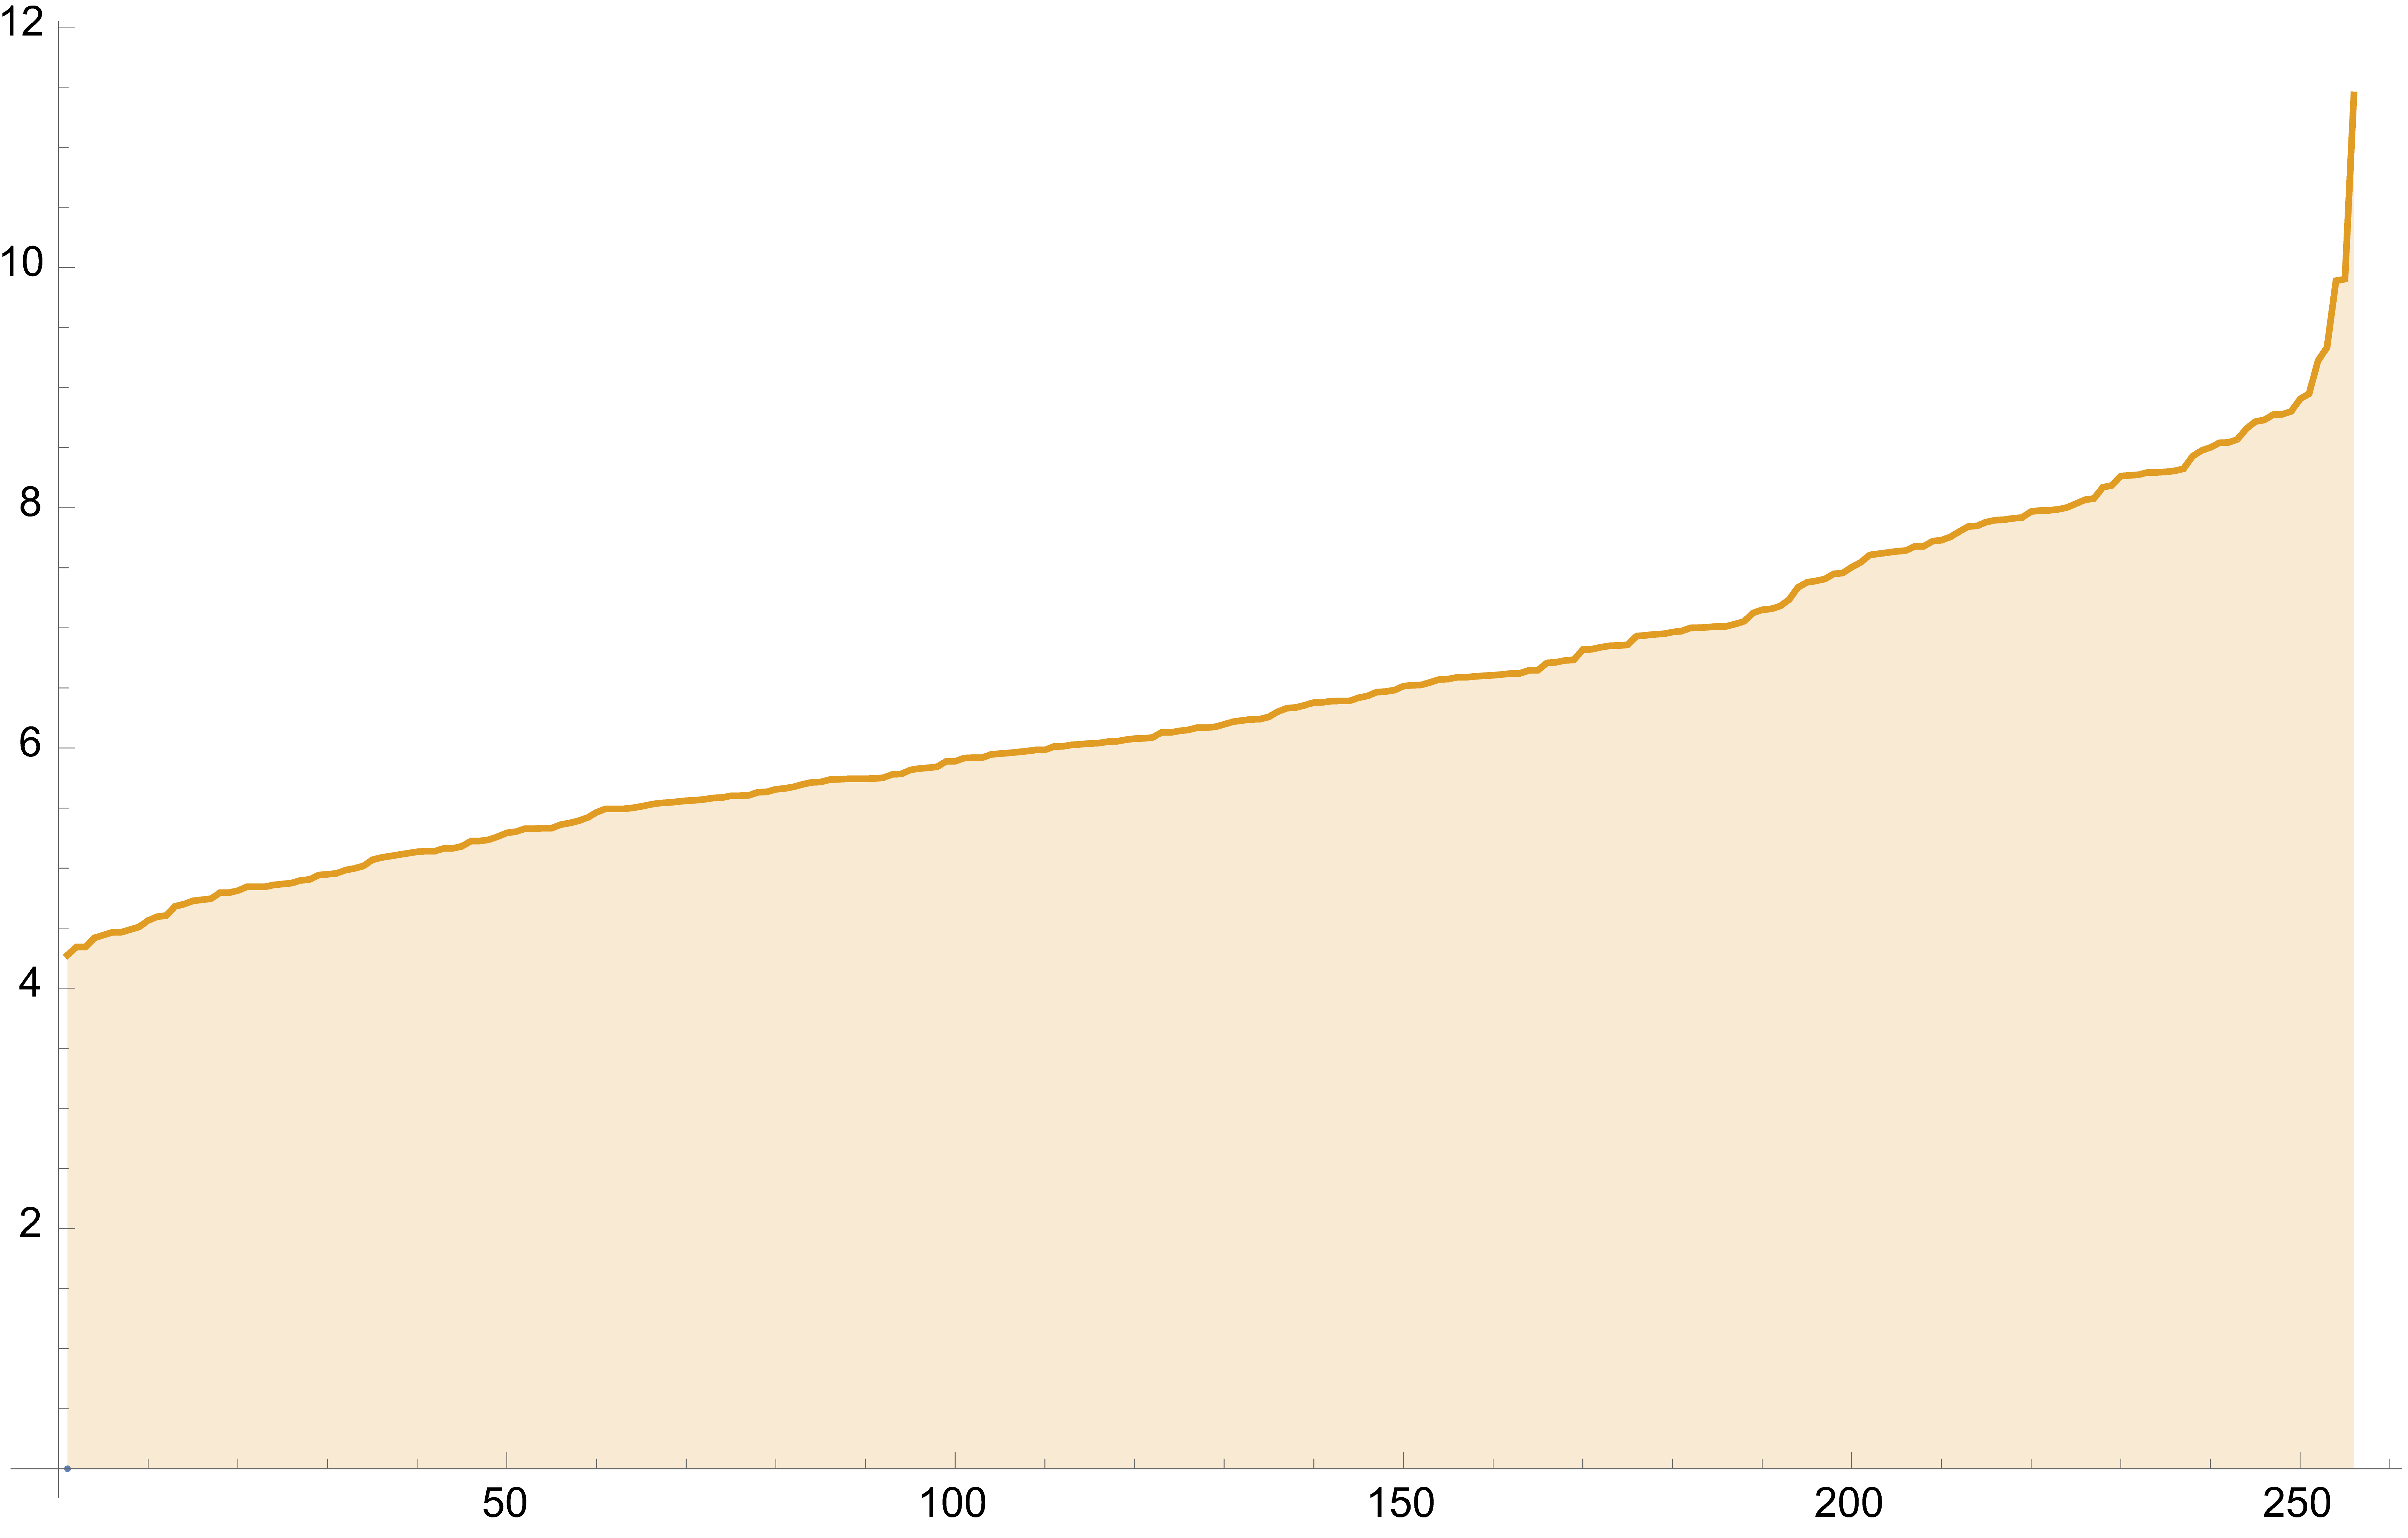
\includegraphics[scale=0.7]{historygramorig2}
    \caption*{Histograma de los bytes del archivo cifrado.}
    \label{fig:d3}
\end{figure}

\begin{figure}[H]
    \centering
    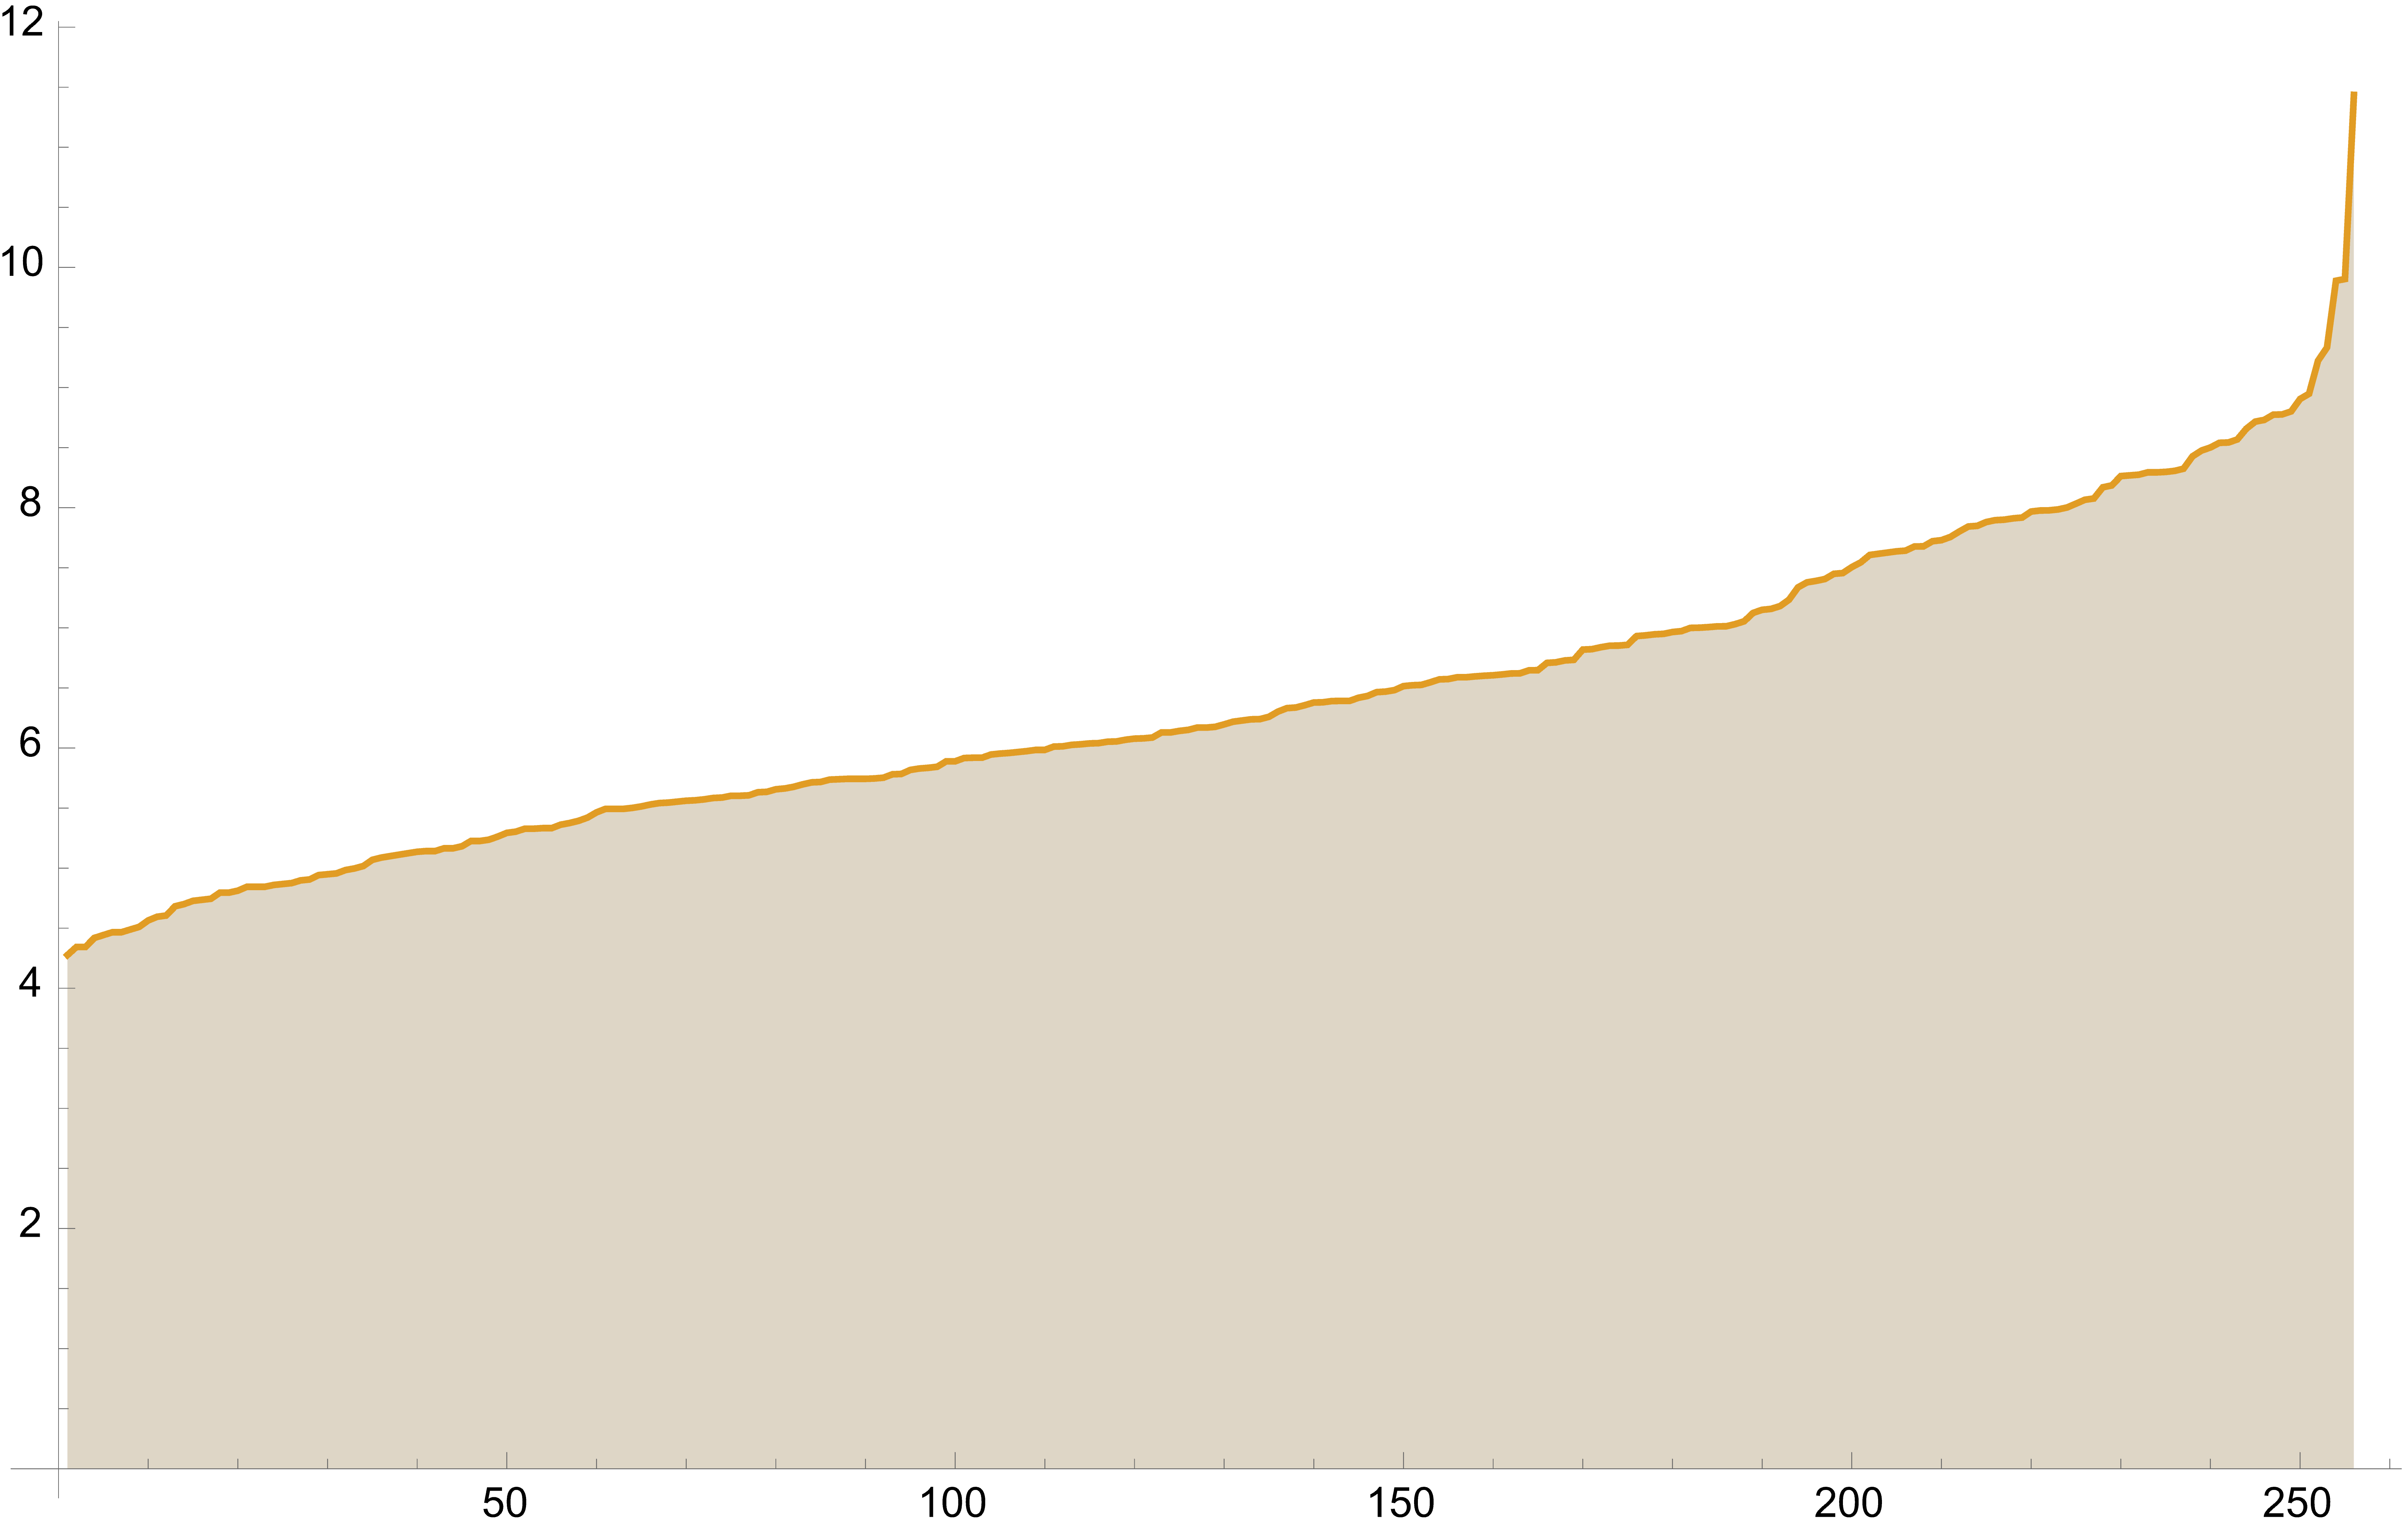
\includegraphics[scale=0.7]{historygram}
    \caption*{Histograma de los bytes del archivo
original y el cifrado.}\label{fig:d2}
\end{figure}

Graficas elaboradas en Mathematica 13 con el código:

\begin{minted}[linenos]{wolfram}
Show[
    With[
        {
            assoc = CountRepetitions[baa],
            assoc2 = CountRepetitions[Flatten[bx]]
        },

        ListLinePlot[
            {
                KeyValueMap[Log[#2] &]@KeySortBy[assoc, assoc[#] &],
                KeyValueMap[Log[#2] &]@KeySortBy[assoc2, assoc2[#] &]
            },
            Filling -> Axis,
            PlotRange -> Full,
            ImageSize -> Large
        ]
    ]
]
\end{minted}

donde \texttt{baa} es un arreglo de bytes conteniendo el estado del archivo
original y donde \texttt{bx} es una matriz que se usa como arreglo de bytes que
contiene el estado cifrado de los contenidos de donde \texttt{baa}.

\end{document}